\documentclass[a4paper]{article}
\usepackage[utf8]{inputenc}
\usepackage[russian,english]{babel}
\usepackage[T2A]{fontenc}
\usepackage[left=10mm, top=20mm, right=18mm, bottom=15mm, footskip=10mm]{geometry}
\usepackage{indentfirst}
\usepackage{amsmath,amssymb}
\usepackage[italicdiff]{physics}
\usepackage{graphicx}
\usepackage{multirow}
\usepackage{svg}
\graphicspath{{images/}}
\DeclareGraphicsExtensions{.pdf,.png,.jpg}
\usepackage{wrapfig}
\usepackage{caption}
\usepackage[table,xcdraw]{xcolor}
\captionsetup[figure]{name=Рисунок}
\captionsetup[table]{name=Таблица}

\begin{document}

\title{\underline{Свободные и вынужденные колебания в электрическом контуре}}
\author{Каспаров Николай, Б01-304}

\maketitle

\paragraph*{Цель работы:} исследование свободных и вынужденных колебаний в
колебательном контуре.

\paragraph*{В работе используются:} осциллограф АКТАКОМ ADS-6142H, генератор сигналов специальной формы АКИП-3409/4, магазин сопротивления МСР-60, магазин емкости Р5025, магазин индуктивности Р567 типа
МИСП, соединительная коробка с шунтирующей емкостью, соединительные одножильные и коаксиальные провода.

\section{Ход работы}

\subsection{Измерение периодов свободных колебаний}

Соберем установку, выставим $R \approx 0$ Ом, $L=100.0 \pm 0.1$ мГн, $C \approx 0$ нФ

Вычислим величину емкости $C_0$ самой установки:

$T_0 = 2\pi \sqrt{LC_0} \longrightarrow C_0 = \frac{T^2}{4\pi^2L} = (1.24 \pm 0.04) \ \text{нФ} $
	
Будем увеличивать емкость контура и сравнивать экспериментальную величину периода с вычисленной теоретически: 

\begin{table}[h!]
\centering
\begin{tabular}{|c|c|c|}
\hline
\multicolumn{1}{|l|}{C, нФ} & \multicolumn{1}{l|}{$T^\text{эксп}$, \text{мс}} & \multicolumn{1}{l|}{T^\text{теор}, \text{мс}} \\ \hline
1 & $0.09 \pm 0.01$ & 0.09 \\ \hline
2 & $0.11 \pm 0.01$ & 0.11 \\ \hline
4 & $0.14 \pm 0.01$ & 0.14 \\ \hline
6 & $0.17 \pm 0.01$ & 0.17 \\ \hline
8 & $0.19 \pm 0.01$ & 0.19 \\ \hline
9 & $0.20 \pm 0.01$ & 0.20 \\ \hline
\end{tabular}
\end{table}

\subsection{Критическое сопротивление и декремент затухания}

Подберем и установим значение $C^*$ так, 
чтобы частота собственных колебаний была 
$\nu_0 = 6.5$ кГц. 

\noindent
$C^* = \frac{1}{4\pi^2\nu_0^2L} \approx 6$ нФ. Рассчитаем теоретически критическое сопротивление контура $R_{cr} = 2\sqrt{\frac{L}{C}} \approx 8168$ Ом.
Измеряем логарифмических декремент затухания по соседним максимумам при различных внешних сопротивлениях ($0,05 R_{cr} - 0,2R_{cr}$):

\begin{table}[h!]
\centering
\begin{tabular}{|c|c|c|c|}
\hline
\multicolumn{1}{|l|}{R, Ом} & \multicolumn{1}{l|}{R + R\_L, Ом} & \multicolumn{1}{l|}{$\theta$ = $U_k/U_{k+1}$} & \multicolumn{1}{l|}{Q = $\pi/\theta$} \\ \hline
400  & 430  & 0.40 & $ 7.94 \pm 0.11$\\ \hline
800  & 830  & 0.67 & $ 4.67 \pm 0.07$\\ \hline
1200 & 1230 & 1.00 & $ 3.15 \pm 0.04$\\ \hline
1600 & 1630 & 1.26 & $ 2.49 \pm 0.04$\\ \hline
2000 & 2030 & 1.34 & $ 2.35 \pm 0.03$\\ \hline
\end{tabular}
\end{table}

\begin{figure}[h!]
\centering
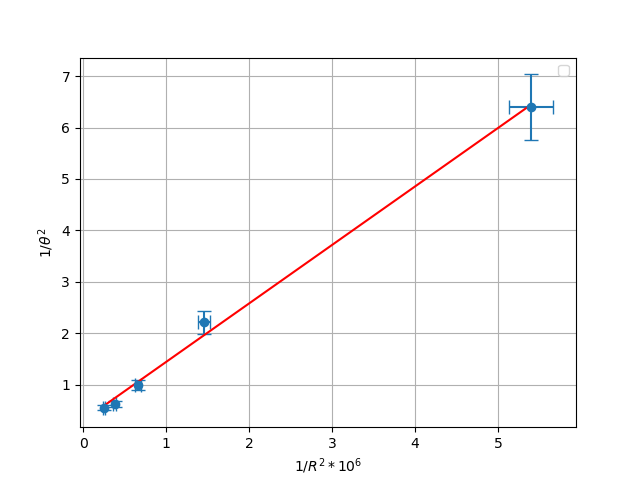
\includegraphics[width=0.8\textwidth]{Figure_1.png}
\caption{График зависимости логарифмического коэффициента затухания от сопротивления}
\end{figure}

Коэффициент $k = 1.1 \pm 0.1$, экспериментально определяем $R_{cr} = 2 \pi \sqrt{k} = 6.7 \pm 0.6 $ кОм.
Значение совпадает в $3 \sigma$ с полученным напрямую.

\subsection{Свободное колебание на фазовой плоскости}

C помощью осциллографа получаем портрет колебаний на фазовой плоскости,
определяем декремент затухания по соседним пересечениям оси X.

\begin{table}[h!]
\centering
\begin{tabular}{|c|c|c|c|c|}
\hline
\multicolumn{1}{|c|}{$R$, Ом} & \multicolumn{1}{c|}{$U_k$, дел} & \multicolumn{1}{c|}{$U_{k+1}$, дел} & \multicolumn{1}{c|}{$\theta$} & \multicolumn{1}{c|}{Q} \\ \hline
430                         & 3.4                             & 2.2                                 & 0.44                          & 7.2                    \\ \hline
2030                        & 3.2                             & 0.4                                 & 2.08                          & 1.5                    \\ \hline
\end{tabular}
\end{table}

Рассчитаем теоретическое значение добротности через параметры контура
\[Q = \frac{\pi}{\theta} = \frac{\pi}{\gamma T} = \frac{\pi}{\frac{R}{2L}\frac{2\pi}{\omega_1}} = \frac{L}{R}\omega_1 = \frac{L}{R}\sqrt{\omega_0^2 - \gamma^2} = \frac{L}{R}\sqrt{\frac{1}{LC} - \frac{R^2}{4L^2}} = \frac{1}{2}\sqrt{\frac{4L}{CR^2} - 1}\]

При параметрах $L = 100$ мГн, $C = 6$ нФ имеем :

1. $R_1 =  440$ Ом \qquad $Q_1 = 9.5 \pm 0.2$,

2. $R_2 = 2030$ Ом \qquad $Q_2 = 1.95 \pm 0.05$,

\newpage

\subsection{Измерение АЧХ и ФЧХ вынужденных колебаний}

\begin{figure}[h!]
\centering
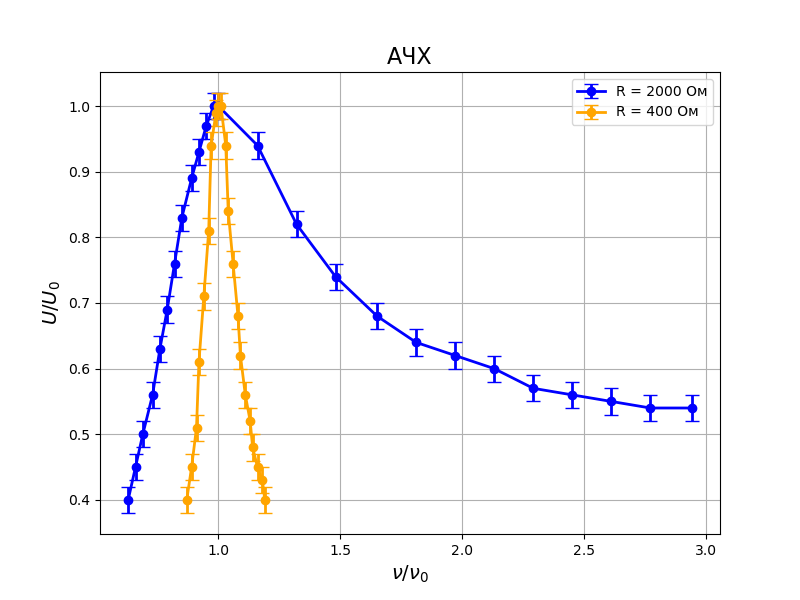
\includegraphics[width=0.8\textwidth]{Figure_2.png}
\caption{Амплитудно-Частотная характеристика колебаний}
\end{figure}

\begin{figure}[h!]
\centering
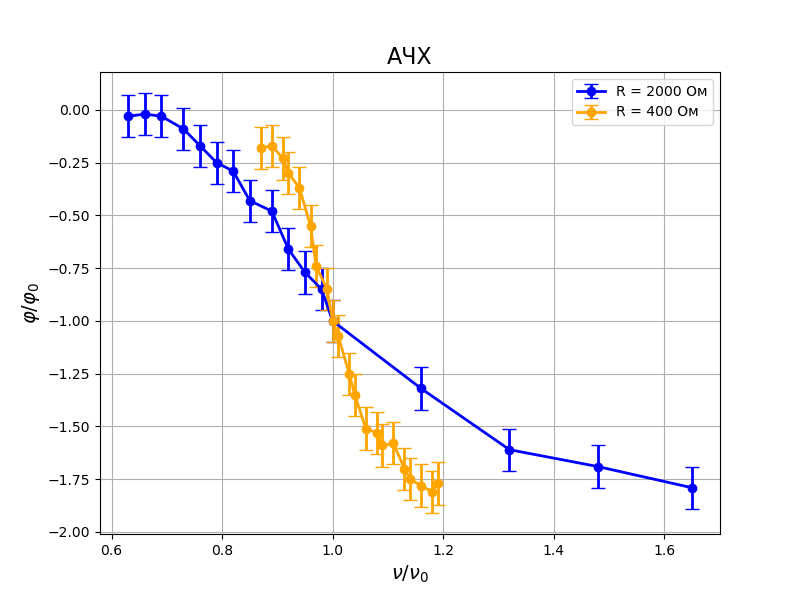
\includegraphics[width=0.8\textwidth]{Figure_3.png}
\caption{Фазово-Частотная характеристика колебаний}
\end{figure}

\noindent Определим добротность по графику АЧХ. 
$Q = \frac{\omega_0}{2\Delta \Omega}$, где $2\Delta \Omega$ - ширина резонансной кривой на уровне $U = \frac{U_0}{\sqrt{2}}$.
	
\noindent Рассчитаем добротность по ФЧХ. 
Для этого проведем горизонтальную линию через уровень, где наблюдается резонанс.
Затем отразим одну половину относительно этой прямой и измерим приблизительно ширину на расстоянии $\frac{\pi}{4}$ от резонанса.

\noindent Данные занесём в таблицу:

\begin{table}[h!]
    \centering
\begin{tabular}{|c|cc|cc|}
\hline
Метод    & \multicolumn{2}{c|}{АЧХ}        & \multicolumn{2}{c|}{ФЧХ}        \\ \hline
R, Ом    & \multicolumn{1}{c|}{400} & 2000 & \multicolumn{1}{c|}{400} & 2000 \\ \hline
Q        & \multicolumn{1}{c|}{7.6} & 1.30 & \multicolumn{1}{c|}{9.1} & 2.8  \\ \hline
\end{tabular}
\end{table}

\section{Вывод}

В данной лабораторной работе мы исследовали колебания в электрическом контуре и 
различными способами нашли его добротность. Наилучшую погрешность дал метод, 
использующий декремент затухания. Хуже всего показал себя метод фазовой спирали.

\end{document}

